\chapter{Część kliencka aplikacji}

Część kliencka naszej aplikacji została oparta o javascriptowy framwork Ext JS. Jest to rozbudowany pakiet do tworzenia nowoczesnych aplikacji internetowych. Udostępnia funkcje do zarządzania elementami drzewa DOM, oraz szereg własnych komponentów graficznych tj. panele, tabelki, formularze etc. Biblioteka posiada również szerokie wsparcie dla technologii AJAX. Ext JS został stworzony z myślą o tworzeniu rozbudowanych aplikacji i dlatego twórcy pomyśleli o architekturze, która pozwoli w naturalny i logiczny sposób zorganizować kod programu. Struktura aplikacji opiera się o schemat MVC. Twórcy Ext JS zalecają pewien schemat hierarchii katalogów uwzględniający podział projektu na warstwy. Przykład organizacji aplikacji:

\begin{figure}[H]
	\centering
	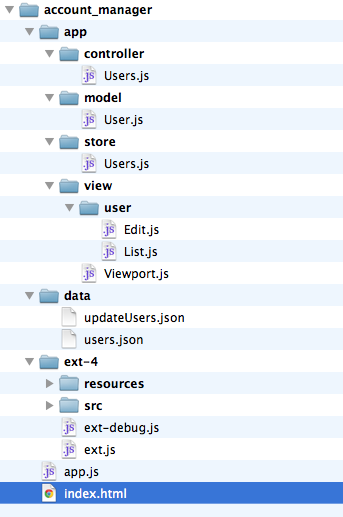
\includegraphics[scale=0.5]{images/struktura_folderow.png}
	\caption{Struktura folderów aplikacji}
\end{figure}

\section{Warstwa modelu}

Definiuje klasy będące odwzorowaniem klas języka Java, które otrzymujemy w odpowiedzi od serwera. W klasach modelu wykonujemy konwersję surowych danych do czytelnego formatu jeżeli jest taka potrzeba. Na tym poziomie możemy również wprowadzić walidację pól. Ext JS wspiera architekturę REST dzięki temu w klasach modelu podając adres URL do zasobów otrzymamy gotowe funkcje zapisu, odczytu, modyfikacji i usuwania danych. Przeanalizujmy przykład z naszego projektu:

\begin{figure}[H]
	\centering
	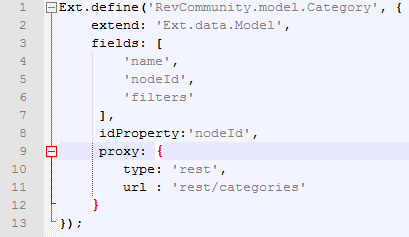
\includegraphics[width=\textwidth]{images/ext_model.png}
	\caption{Przykład definicji modelu w Ext JS}
\end{figure}

Powyższy kod implementuje klasę modelu Category. Dzięki definicji obiektu proxy zarządzanie naszymi danymi staje się banalnie proste. Przykładowo w celu zapisania nowej kategorii wystarczy:

\begin{figure}[H]
	\centering
	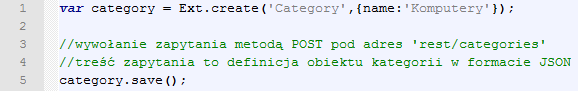
\includegraphics[width=\textwidth]{images/save_model.png}
	\caption{Zapis obiektu poprzez klasę modelu}
\end{figure}

Jeżeli wykonamy metodę save na obiekcie, który posiada już przypisany identyfikator(w naszym przypadku pole nodeId), to metodą zapytania będzie PUT.
Do dyspozycji mamy również metody destroy(usuwanie elementu), oraz load(pobieranie elemntu).

Kolejnym elementem zaliczającym się do tej warstwy są klasy Store służące do zarządzania grupami obiektów. Wykorzystuje się je przy ładowaniu danych do komponentów np. tabel. 
Klasy Store pozwalają również filtrować i sortować dane.

\section{Warstwa widoku}

Na widok aplikacji składają się komponenty graficzne tj. panele, tabele, drzewa i formularze. Biblioteka pozwala nam rozszerzać komponenty graficzne tworząc własne, dzięki temu możemy je dostosować do własnych potrzeb i wykorzystywać w wielu miejscach(również w innych aplikacjach). Bardzo przydatnym elementem Ext JS jest mechanizm szablonów(Ext.XTemplate). Pozwala on tworzyć wygląd komponentów z wykorzystaniem języka HTML i specjalnych znaczników framework'a Ext JS. Zazwyczaj szablony służą do definicji wyglądu list elementów. Komponent, w którym używamy szablonu wiążemy z konkretnym modelem. Gdy spróbujemy załadować dane do komponentu model wywoła odpowiednie zapytanie do serwera w celu pobrania danych. Następnie zwrócona kolekcja zostanie przetworzona przez szablon. W szablonie możemy odwoływać się do pól modelu, iterować po kolekcjach elementów, oraz wykorzystywać warunki logiczne. Spójrzmy na prosty przykład szablonu listy subskrybowanych użytkowników:
 
\begin{figure}[H]
	\centering
	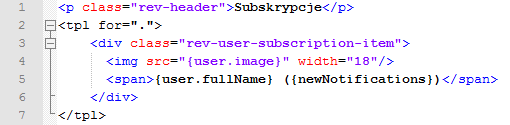
\includegraphics[width=\textwidth]{images/tpl.png}
	\caption{Szablon listy subskrybowanych użytkowników}
\end{figure}

Widok naszego komponentu w całości definiuje powyższy szablon. Zaczynamy od wstawienia nagłówka "Subskrypcje" jako zwykły paragraf HTML. Niżej widzimy znacznik 'tpl', który udostępnia rozszerzenia szablonów. W tym przypadku będziemy iterować po kolekcji elementów załadowanej do komponentu. Następnie mamy definicje elementów HTML zawierających znaczniki odwołujące się do pól modelu. Jednym z pól modelu jest obiekt user. Możemy odwoływać się do jego właściwości poprzez znak '.'. W połączeniu z definicją stylów CSS otrzymujemy następujący efekt:

 


\section{Warstwa kontrolerów}

Aby nasza aplikacja zaczęła "żyć" musimy zdefiniować zachodzące w nie zdarzenia i ich obsługę. Do tego służą kontrolery. Są to klasy w których umieszczamy instrukcję w typu: gdy na komponencie ... wydarzy się ... wykonaj ... . Przykładowo w kontrolerach umieszczamy obsługę kliknięć przycisków, zdarzeń załadowania danych, lub edycji pól formularzy. Ciekawy jest sposób wiązania komponentu z funkcją obsługi zdarzenia. Pierwszą istotną rzeczą, którą musimy wykonać to zidentyfikowanie komponentu dla którego będziemy definiować zdarzenie. Do tego celu wykorzystujemy mechanizm Ext Js - ComponentQuery. Jest to język zapytań pozwalający na wyszukiwanie komponentów na podstawie aliasów, identyfikatorów, powiązań z innymi komponentami, oraz wartości ich atrybutów. Każda klasa powinna posiadać unikalny w ramach aplikacji alias. Alias ten upraszcza tworzenie obiektów danej klasy(nie musimy podawać pełnej nazwy klasy), oraz znacznie ułatwia tworzenie zapytań. Spójrzmy na przykład: 

\begin{figure}[H]
	\centering
	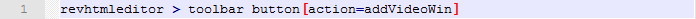
\includegraphics[width=\textwidth]{images/cmp_query.png}
	\caption{Zapytanie Ext.ComponentQuery}
\end{figure}

Zapytanie zostanie przetworzone w następujący sposób:

\begin{itemize}
\item wyszukanie wszystkich komponentów na stronie posiadających alias 'revhtmleditor'
\item wśród bezpośrednich dzieci znalezionych wcześniej komponentów wybierzemy tylko elementy typu toolbar ( gdyby nie znak '>' wyszukiwanie zagłębiałoby się rekurencyjnie)
\item w znalezionych toolbar'ach szukamy tylko przycisków, mających atrybut action ustawiony na wartość addVideoWin
\end{itemize}

Tak elastyczny mechanizm wyszukiwania pozwala znaleźć każdy komponent.
Kolejnym krokiem jest wybranie zdarzenia dla znalezionego komponentu. Ext Js określił dla każdego komponentu wyczerpującą listę dostępnych zdarzeń. Naszym zadaniem jest ich przypisanie do funkcji javascriptowych i implementacji obsługi.

Naszym rozszerzeniem powyższej architektury jest dodanie warstwy usług, której zadanie jest analogiczne do jej serwerowego odpowiednika. Stworzenie klas usług po stronie klienta miało na celu wyciągniecie implementacji z klas kontrolerów po to, aby lepiej zorganizować kod i umożliwić korzystanie z przydatnych funkcji w wielu miejscach. Pamiętajmy, że kontrolery są mocno związane z komponentami, natomiast klasy usług są podzielone według obszaru, którego dotyczą np. produktów, recenzji. Dlatego kontrolery zajmują się przetworzeniem danych do odpowiedniego formatu wymaganego przez klasy usług, nie implementują bezpośrednio żadnych operacji.




\section{Dynamiczne style CSS}
W projekcie do opisu formy prezentacji widoku strony klienckiej użyto dynamicznych arkuszy stylów – LESS. Głównym zadaniem LESS jest rozszerzenie możliwości CSS (ang. Cascading Style Sheets) między innymi o takie elementy jak możliwość definiowania zmiennych i funkcji, łatwe zagnieżdżanie selektorów czy proste operacje. Wszystko to zostaje później podczas ładowania strony przekompilowane na zwykły kod CSS, tak by był on zrozumiały dla przeglądarek. CSS czyli kaskadowy arkusz styli pozwala dodać graficzny układ do strony internetowej. Określają one wygląd różnych elementów HTML znajdujących się na danej stronie internetowej. 
LESS ma przewagę nad CSS, ponieważ zmienne pozwalają na zdefiniowanie wartości na przykład koloru czy szerokości w jednym miejscu, które następnie można wykorzystać w obrębie całego arkusza stylów. Umożliwia to globalne zmiany poprzez modyfikację jednej linijki kodu. Jest to bardzo wygodne rozwiązanie. 

\begin{figure}[h]
	\centering
	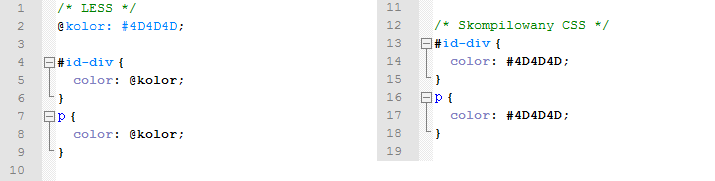
\includegraphics[width=1.00\textwidth]{images/less1.png}
	\caption{Przykładowy kod LESS i wygenerowany z niego kod CSS}
\end{figure}
\paragraph{}
W zwykłym pliku CSS, gdy jest potrzeba zmiany na przykład jakiegoś koloru na inny, trzeba ręcznie tą wartość zmienić w każdym miejscu arkusza stylów, w którym się pojawia. Jest to czasochłonne, dlatego przy budowie projektu zrezygnowano z tego rozwiązania na rzecz LESS. 
W dynamicznych arkuszach styli można tworzyć również tak zwane „domieszki”. Domieszki to inaczej dziedziczenie przez dopisanie wartości do wszystkich właściwości danej klasy w innej klasie, poprzez wykorzystanie nazwy klasy jako jednej z wartości innej klasy. Zasada działania jest podoba do zmiennych, przy czym domieszki dotyczą całej konkretnej klasy. Domieszki mogą również działać jak funkcje i przyjmować argumenty, tak jak w poniższym przykładzie.

\begin{figure}[h]
	\centering
	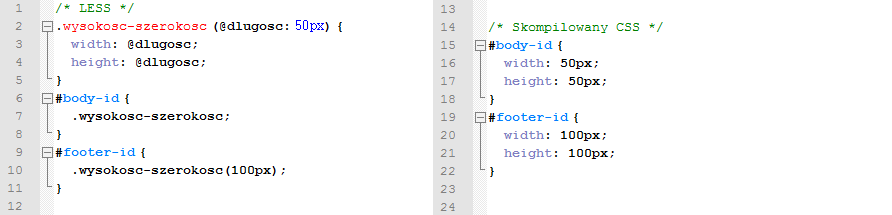
\includegraphics[width=1.00\textwidth]{images/less2.png}
	\caption{Przykład użycia domieszek}
\end{figure}
\paragraph{}

Dynamiczny arkusz styli  będąc rozszerzeniem kaskadowego arkusza styli jest z nim zarówno kompatybilny wstecz jak i korzysta z jego składni w czasie budowy nowych struktur leksykalnych. To sprawia, że nauka LESS jest prosta.
W projekcie kompilacja plików LESS do plików CSS następuje wraz z restartem serwera, dzięki czemu ten zabieg nie obciąża użytkowników. \cite{LESS}


\section{AJAX}
Wykorzystanie biblioteki Ext JS do budowy klienckiej części aplikacji, umożliwiło realizację projektu w oparciu o koncepcję AJAX (Asynchronous JavaScript and XML). Jest to technika tworzenia aplikacji internetowych, w której komunikacja pomiędzy klientem, zrealizowanym w języku JavaScript, a serwerem odbywa się asynchronicznie, dzięki czemu nie ma konieczności przeładowania całej strony w celu zmiany jej treści, a użytkownik może kontynuować pracę, oczekując na odpowiedź z serwera.\cite{ajaxWoj}

Zastosowanie asynchronicznych wywołań sprawdza się doskonale podczas ładowania danych do graficznych komponentów warstwy widoku, takich jak panele, listy czy tabele. W trakcie pobierania danych do jednego z komponentów, pozostała część strony pozostaje aktywna i umożliwia interakcję z użytkownikiem, w tym także realizację kolejnych zapytań. Ponadto, po zakończeniu ładowania aktualizowane są tylko te elementy strony, dla których jest to konieczne. Wszystko to, ma pozytywny wpływ na poziom interaktywności i wrażenia końcowego użytkownika aplikacji.

Najważniejsze zastosowania techniki AJAX w aplikacji revCommunity:

\begin{itemize}
\item\textbf{Dynamiczne drzewo kategorii.} Ze względu na nieograniczone możliwości rozbudowy drzewa kategorii, komponent ten został zorganizowany w taki sposób, by żądane elementy pobierać tylko wtedy, gdy zachodzi konieczność ich prezentacji.
\begin{figure}[h]
	\centering
	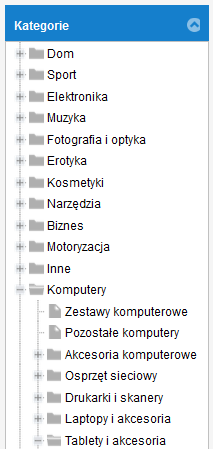
\includegraphics[scale=0.7]{images/Kategorie.png}
	\caption{Dynamiczne drzewo kategorii}
\end{figure}
\item\textbf{Stronicowanie (ang. paging) i sortowanie.} Ze względu na nieograniczone możliwości rozbudowy drzewa kategorii, komponent ten został zorganizowany w taki sposób, by żądane elementy pobierać tylko wtedy, gdy zachodzi konieczność ich prezentacji.
\begin{figure}[h]
	\centering
	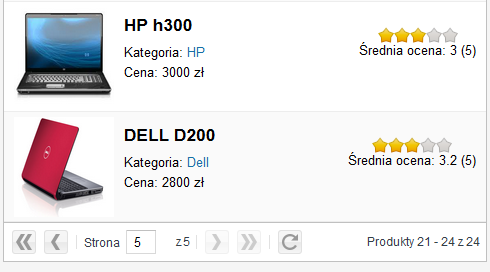
\includegraphics[scale=0.7]{images/paging.png}
	\caption{Stronicowanie listy produktów}
\end{figure}
\item\textbf{Współbieżne ładowanie danych przez komponenty widoku.} Przykładem takiego zastosowania techniki AJAX jest ekran startowy aplikacji, w którym zarówno lista produktów, lista recenzji, jak i widok polecanych użytkowników ładowane są niezależnie.
\begin{figure}[h]
	\centering
	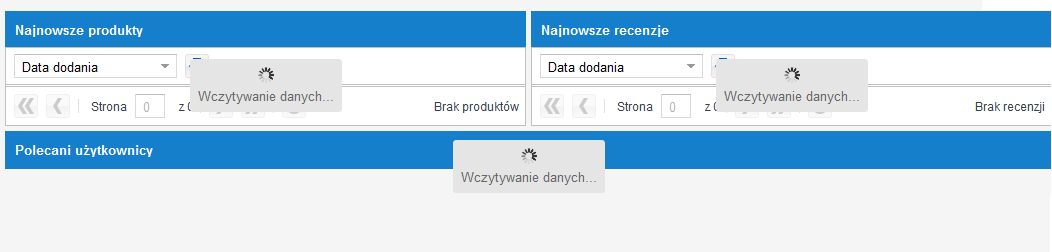
\includegraphics[scale=0.7]{images/Loading.png}
	\caption{Współbieżne ładowanie danych}
\end{figure}
\end{itemize}


Warto także zwrócić uwagę na wady stosowania techniki AJAX. Najważniejszą z nich jest porzucenie tradycyjnego schematu przeglądania stron z wykorzystaniem przycisków ,,wstecz'' i ,,dalej'' w oknie przeglądarki. Wywołanie akcji powodującej modyfikację części zawartości strony nie modyfikuje adresu URL i nie jest rejestrowane przez mechanizm historii przeglądarki. Dodatkowo, powoduje to, że poszczególne widoki aplikacji, takie jak szczegóły produktu czy lista produktów nie są dostępne pod określonym adresem URL. Pozostaje on niezmieniony przez cały cykl życia aplikacji.\cite{jsadv}

Wspomniany problem można jednak rozwiązać przy wykorzystaniu dodatkowych narzędzi. Jednym z nich jest biblioteka Backbone.js umożliwiająca wykorzystanie alternatywnej metody zarządzania historią i adresami url w aplikacji internetowej wykorzystującej AJAX. Idea opiera się, na wykorzystaniu w adresie url znaku \# (ang. hashtag), którego dodanie do istniejącego adresu nie powoduje przeładowania strony.\cite{urls} Obiekt Backbone.Router analizuje tekst znajdujący się za znakiem \# i na podstawie zdefiniowanych przez programistę reguł wywołuje jedną z zaimplementowanych funkcji. W systemie revCommunity, funckje te zostały wykorzystane do sterowania widokami aplikacji.\cite{backbone}

Przykłady reguł routingu w aplikacji revCommunity:

\begin{lstlisting}
routes : {
	'':'home',
	'category/new':'newCategory',
	'products/filter/:categoryId':'filterProducts',
	'products/:id':'product',
	'reviews/:id':'review',
},
\end{lstlisting}

Każda reguła zbudowana jest według schematu [wzorzec] : [nazwa\_funkcji]. W momencie zmiany adresu url w przeglądarce, pobierana jest jego część znajdująca się za znakiem \textbf{\#}, która następnie poddawana jest próbie dopasowania do kolejnych wzorców. W przypadku udanego przypasowania, wywoływana jest funkcja o nazwie podanej w drugiej części reguły.

Wzorzec może zawierać dodatkowo specjalne wyrażenia ułatwiające manipulację adresami. Jednym z nich jest użyta w powyższym przykładzie konstrukcja \textit{'products/filter/:categoryId':'filterProducts'}, dzięki której część dopasowanego adresu url, znajdująca się w miejscu identyfikatora \textit{':categoryId'} zostanie przekazana do funkcji \textit{filterProducts} jako argument o nazwie \textit{categoryId}.

Warto również zauważyć, że kolejność reguł ma wpływ na ich późniejszą interpretację. Biblioteka Backbone.js przegląda reguły w kolejności ich definiowania. W powyższym przykładzie reguła \textit{'products/filter/:categoryId':'filterProducts'} celowo została umieszczona przed regułą \textit{'products/:id':'product'}, poniważ jej wzorzec \textit{'products/filter/:categoryId'} zawiera się we wzorcu \textit{'products/:id'}. Zamiana kolejności wspomnianych reguł spowodowałaby brak możliwości wykorzystania jednej z nich.\cite{backbone}